% GNUPLOT: LaTeX picture with Postscript
\begingroup
  \makeatletter
  \providecommand\color[2][]{%
    \GenericError{(gnuplot) \space\space\space\@spaces}{%
      Package color not loaded in conjunction with
      terminal option `colourtext'%
    }{See the gnuplot documentation for explanation.%
    }{Either use 'blacktext' in gnuplot or load the package
      color.sty in LaTeX.}%
    \renewcommand\color[2][]{}%
  }%
  \providecommand\includegraphics[2][]{%
    \GenericError{(gnuplot) \space\space\space\@spaces}{%
      Package graphicx or graphics not loaded%
    }{See the gnuplot documentation for explanation.%
    }{The gnuplot epslatex terminal needs graphicx.sty or graphics.sty.}%
    \renewcommand\includegraphics[2][]{}%
  }%
  \providecommand\rotatebox[2]{#2}%
  \@ifundefined{ifGPcolor}{%
    \newif\ifGPcolor
    \GPcolortrue
  }{}%
  \@ifundefined{ifGPblacktext}{%
    \newif\ifGPblacktext
    \GPblacktextfalse
  }{}%
  % define a \g@addto@macro without @ in the name:
  \let\gplgaddtomacro\g@addto@macro
  % define empty templates for all commands taking text:
  \gdef\gplbacktext{}%
  \gdef\gplfronttext{}%
  \makeatother
  \ifGPblacktext
    % no textcolor at all
    \def\colorrgb#1{}%
    \def\colorgray#1{}%
  \else
    % gray or color?
    \ifGPcolor
      \def\colorrgb#1{\color[rgb]{#1}}%
      \def\colorgray#1{\color[gray]{#1}}%
      \expandafter\def\csname LTw\endcsname{\color{white}}%
      \expandafter\def\csname LTb\endcsname{\color{black}}%
      \expandafter\def\csname LTa\endcsname{\color{black}}%
      \expandafter\def\csname LT0\endcsname{\color[rgb]{1,0,0}}%
      \expandafter\def\csname LT1\endcsname{\color[rgb]{0,1,0}}%
      \expandafter\def\csname LT2\endcsname{\color[rgb]{0,0,1}}%
      \expandafter\def\csname LT3\endcsname{\color[rgb]{1,0,1}}%
      \expandafter\def\csname LT4\endcsname{\color[rgb]{0,1,1}}%
      \expandafter\def\csname LT5\endcsname{\color[rgb]{1,1,0}}%
      \expandafter\def\csname LT6\endcsname{\color[rgb]{0,0,0}}%
      \expandafter\def\csname LT7\endcsname{\color[rgb]{1,0.3,0}}%
      \expandafter\def\csname LT8\endcsname{\color[rgb]{0.5,0.5,0.5}}%
    \else
      % gray
      \def\colorrgb#1{\color{black}}%
      \def\colorgray#1{\color[gray]{#1}}%
      \expandafter\def\csname LTw\endcsname{\color{white}}%
      \expandafter\def\csname LTb\endcsname{\color{black}}%
      \expandafter\def\csname LTa\endcsname{\color{black}}%
      \expandafter\def\csname LT0\endcsname{\color{black}}%
      \expandafter\def\csname LT1\endcsname{\color{black}}%
      \expandafter\def\csname LT2\endcsname{\color{black}}%
      \expandafter\def\csname LT3\endcsname{\color{black}}%
      \expandafter\def\csname LT4\endcsname{\color{black}}%
      \expandafter\def\csname LT5\endcsname{\color{black}}%
      \expandafter\def\csname LT6\endcsname{\color{black}}%
      \expandafter\def\csname LT7\endcsname{\color{black}}%
      \expandafter\def\csname LT8\endcsname{\color{black}}%
    \fi
  \fi
    \setlength{\unitlength}{0.0500bp}%
    \ifx\gptboxheight\undefined%
      \newlength{\gptboxheight}%
      \newlength{\gptboxwidth}%
      \newsavebox{\gptboxtext}%
    \fi%
    \setlength{\fboxrule}{0.5pt}%
    \setlength{\fboxsep}{1pt}%
    \definecolor{tbcol}{rgb}{1,1,1}%
\begin{picture}(10080.00,5040.00)%
    \gplgaddtomacro\gplbacktext{%
      \csname LTb\endcsname%%
      \put(1342,1100){\makebox(0,0)[r]{\strut{}$0$}}%
      \put(1342,1756){\makebox(0,0)[r]{\strut{}$500000$}}%
      \put(1342,2412){\makebox(0,0)[r]{\strut{}$1\times10^{6}$}}%
      \put(1342,3067){\makebox(0,0)[r]{\strut{}$1.5\times10^{6}$}}%
      \put(1342,3723){\makebox(0,0)[r]{\strut{}$2\times10^{6}$}}%
      \put(1342,4379){\makebox(0,0)[r]{\strut{}$2.5\times10^{6}$}}%
      \put(1905,968){\rotatebox{-45}{\makebox(0,0)[l]{\strut{}Biometric Matching}}}%
      \put(2336,968){\rotatebox{-45}{\makebox(0,0)[l]{\strut{}Biometric Matching (Fast)}}}%
      \put(2767,968){\rotatebox{-45}{\makebox(0,0)[l]{\strut{}Convex Hull}}}%
      \put(3198,968){\rotatebox{-45}{\makebox(0,0)[l]{\strut{}Count 102}}}%
      \put(3630,968){\rotatebox{-45}{\makebox(0,0)[l]{\strut{}Count 10s}}}%
      \put(4061,968){\rotatebox{-45}{\makebox(0,0)[l]{\strut{}Cryptonets (Max Pooling)}}}%
      \put(4492,968){\rotatebox{-45}{\makebox(0,0)[l]{\strut{}Database Join}}}%
      \put(4923,968){\rotatebox{-45}{\makebox(0,0)[l]{\strut{}Database Variance}}}%
      \put(5354,968){\rotatebox{-45}{\makebox(0,0)[l]{\strut{}Histogram}}}%
      \put(5785,968){\rotatebox{-45}{\makebox(0,0)[l]{\strut{}Inner Product}}}%
      \put(6216,968){\rotatebox{-45}{\makebox(0,0)[l]{\strut{}k-means}}}%
      \put(6647,968){\rotatebox{-45}{\makebox(0,0)[l]{\strut{}Longest 102}}}%
      \put(7079,968){\rotatebox{-45}{\makebox(0,0)[l]{\strut{}Max. Dist. b/w Symbols}}}%
      \put(7510,968){\rotatebox{-45}{\makebox(0,0)[l]{\strut{}Minimal Points}}}%
      \put(7941,968){\rotatebox{-45}{\makebox(0,0)[l]{\strut{}MNIST ReLU}}}%
      \put(8372,968){\rotatebox{-45}{\makebox(0,0)[l]{\strut{}Private Set Intersection}}}%
      \put(8935,1100){\makebox(0,0)[l]{\strut{}$0$}}%
      \put(8935,1428){\makebox(0,0)[l]{\strut{}$50$}}%
      \put(8935,1756){\makebox(0,0)[l]{\strut{}$100$}}%
      \put(8935,2084){\makebox(0,0)[l]{\strut{}$150$}}%
      \put(8935,2412){\makebox(0,0)[l]{\strut{}$200$}}%
      \put(8935,2740){\makebox(0,0)[l]{\strut{}$250$}}%
      \put(8935,3067){\makebox(0,0)[l]{\strut{}$300$}}%
      \put(8935,3395){\makebox(0,0)[l]{\strut{}$350$}}%
      \put(8935,3723){\makebox(0,0)[l]{\strut{}$400$}}%
      \put(8935,4051){\makebox(0,0)[l]{\strut{}$450$}}%
      \put(8935,4379){\makebox(0,0)[l]{\strut{}$500$}}%
    }%
    \gplgaddtomacro\gplfronttext{%
      \csname LTb\endcsname%%
      \put(209,2739){\rotatebox{-270}{\makebox(0,0){\strut{}Total Gates}}}%
      \put(9573,2739){\rotatebox{-270}{\makebox(0,0){\strut{}Improvement (number of times)}}}%
      \csname LTb\endcsname%%
      \put(2800,4867){\makebox(0,0)[r]{\strut{}GMW}}%
      \csname LTb\endcsname%%
      \put(2800,4647){\makebox(0,0)[r]{\strut{}GMW (Vectorized)}}%
      \csname LTb\endcsname%%
      \put(5767,4867){\makebox(0,0)[r]{\strut{}BMR}}%
      \csname LTb\endcsname%%
      \put(5767,4647){\makebox(0,0)[r]{\strut{}BMR (Vectorized)}}%
      \csname LTb\endcsname%%
      \put(8734,4867){\makebox(0,0)[r]{\strut{}GMW Improvement}}%
      \csname LTb\endcsname%%
      \put(8734,4647){\makebox(0,0)[r]{\strut{}BMR Improvement}}%
    }%
    \gplbacktext
    \put(0,0){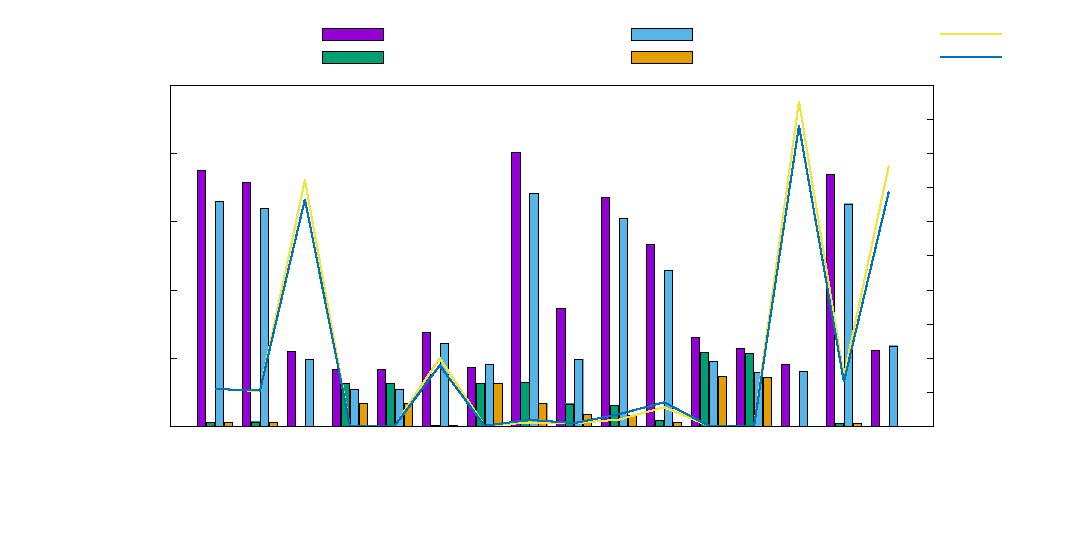
\includegraphics[width={504.00bp},height={252.00bp}]{all-hist-TotalGates}}%
    \gplfronttext
  \end{picture}%
\endgroup
